\section{Task 1: Replay attack on the RF communication} \label{ch:pentesting:replay}
This section details a penetration test against the RF communication between the hardware devices of the system. The specific attack vector explored in this section is a replay attack.

\subsubsection{Background}
A replay attack is an attack in network communication. The attacker listens in on the network traffic and simply retransmits the whole packets or information discovered in the packets to perform authenticated requests against a system they would otherwise not be able to. This type of vulnerability can have devastating consequences since even if several security measures have been taken, such as encrypting the data, the system can still be vulnerable to replay attacks. The attacker needs no knowledge of how the message is structured or what it contains, making it often an easy attack to perform.

Remote Keyless Entry (RKE) systems are notorious for being vulnerable to replay attacks. A famous example is RKE systems in car keys, used to unlock a car with from a distance a press of a button. When these first arrived on the market the security was extremely lacking and researchers in \citeyear{car-rke-systems} found that many cars on the market have used these insecure systems for over 20 years \cite{car-rke-systems}. Often one-way communication from the key to the car over RF signals is used with no protection at all against replay attacks. Simply capturing the RF signal and replaying it would unlock the car, allowing an attacker free access whenever they  please. A simple and well tested protection against replay attacks is sending time-stamps along with your message. If the time stamp is older than some threshold when the receiver would reject the message \cite{rke-replay}. This can, however, sometimes be difficult to implement in embedded systems since it requires both parties to agree on the time. For devices with an internet connection this is easy thanks to the Network Time Protocol (NTP)\footnotelink{https://tools.ietf.org/html/rfc5905}{2021-05-03}. However most low-powered simple IoT devices, such as a car key, does not have internet-connectivity. A solution many modern systems used is a rolling code scheme. Both systems keep an initially synchronized internal code $C$. When the transmitter sends a signal it includes this number and increments it internally. The receiver stores the last such number it received and checks that the number in the new signal is within some interval $[C+1, C+K]$, for some constant $K$. One usually accepts an interval of codes from the last accepted one in case a signal is lost or the button is pressed when you are outside the range of the car. If it is not within that range then the message is rejected. In practice one might use this number to encrypt the message, or use a sequence from a pre-defined pseudo random number generator instead of an integer $C$. This technique protects against replay attacks, however it is still vulnerable against what is called a \textit{rolljam attack} \cite{kamkar2015drive}. By jamming the signal and at the same time recording it the attacker now has a signal they can replay to have one time access to unlock the system. Most modern cars are still susceptible to this type of attack.

\subsubsection{Method} \label{ch:pentesting:replay:method}
The physical setup used during this test is described in section \ref{ch:pentesting:lab-setup}. As stated, a HackRF One SDR was used to receive and transmit RF signals. While low level protocols exist to control the HackRF One, one usually use more higher level tools to interact with it. The method of this test builds on the open source tool \textit{Universal Radio Hacker} (URH), which was created by researchers at Hochschule Stralsund – University of Applied Sciences in Germany \cite{urh}.

Initially, the center frequency at which the system communicates had to be found. This was done using the URH's \textit{Spectrum Analyzer} tool, see figure \ref{fig:finding-center-freq}. In the menu, \textit{HackRF} was selected under devices and the frequency band to listen at was selected. We know from the official documentation that the system communicates at \texttt{868 MHz}, so initially that frequency was set in the menu options. The rest of the parameters were not important and left at their default values. To get the system to transmit data over RF communication, the tamper sensor located on the back of the door sensor was repeatedly pressed and released. While doing this, one could see a clear spike in the frequency spectrum and deduce that the center frequency used by the system is approximately \texttt{868.64 MHz}. This makes sense since the frequency band \texttt{868.6–868.7 MHz} is allocated specifically for alarm systems in Europe \footnotelink{https://en.wikipedia.org/wiki/Short-range_device}{2021-05-14}, as regulated by ETSI \footnotelink{https://www.etsi.org/}{2021-05-14}.
\begin{figure}[!ht]
    \centering
    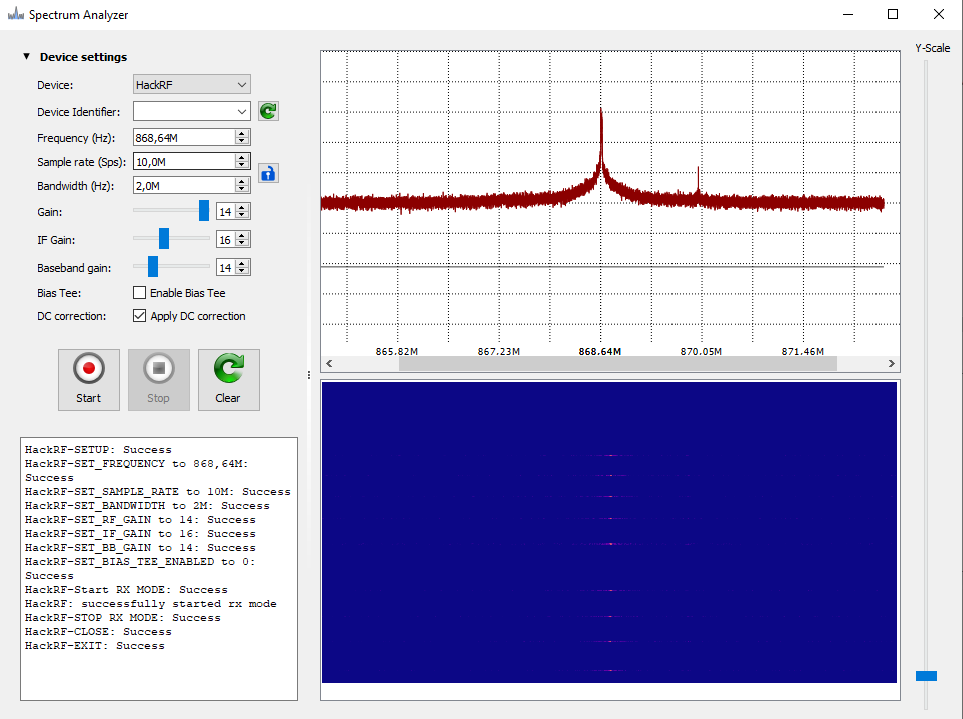
\includegraphics[width=0.9\textwidth]{images/6-pentesting/find-frequency.png}
    \caption{Finding the center frequency of the RF communication.}
    \label{fig:finding-center-freq}
\end{figure}

When the center frequency had been found, signals could be captured using URH's \textit{Record Signal} tool, see figure \ref{fig:rf-signal-capture}. This tool records raw audio signals captures from an SDR. In the menu options, one has to select the correct frequency. After some trial and error, \texttt{868.638 MHz} was found to yield good captured signals. By placing the HackRF close to the devices, the SDR was able to capture clean signals without increasing the gain parameters. See figure \ref{fig:rf-lab-setup} for the physical set up used during this test. By zooming into the captured audio signals and seeing clear sinusoidal waves with a non-trivial pattern, one could verify that the capture was most likely done correctly. Figure \ref{fig:zoomed-in-signal} shows a magnified view of a good signal captured from the door sensor's temper alarm. This was done for all identified communication endpoints of the system.
\begin{figure}[!ht]
    \centering
    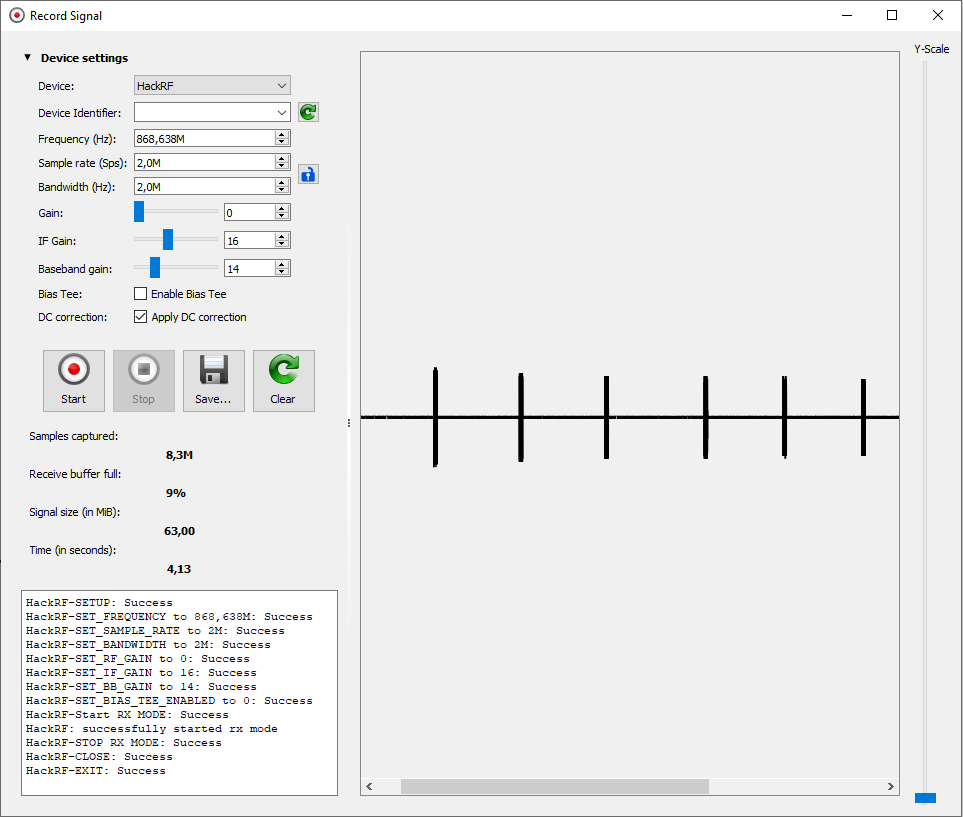
\includegraphics[width=0.9\textwidth]{images/6-pentesting/signal-capture.png}
    \caption{Capturing an RF signal using Universal Radio Hacker.}
    \label{fig:rf-signal-capture}
\end{figure}
\begin{figure}[!ht]
    \centering
    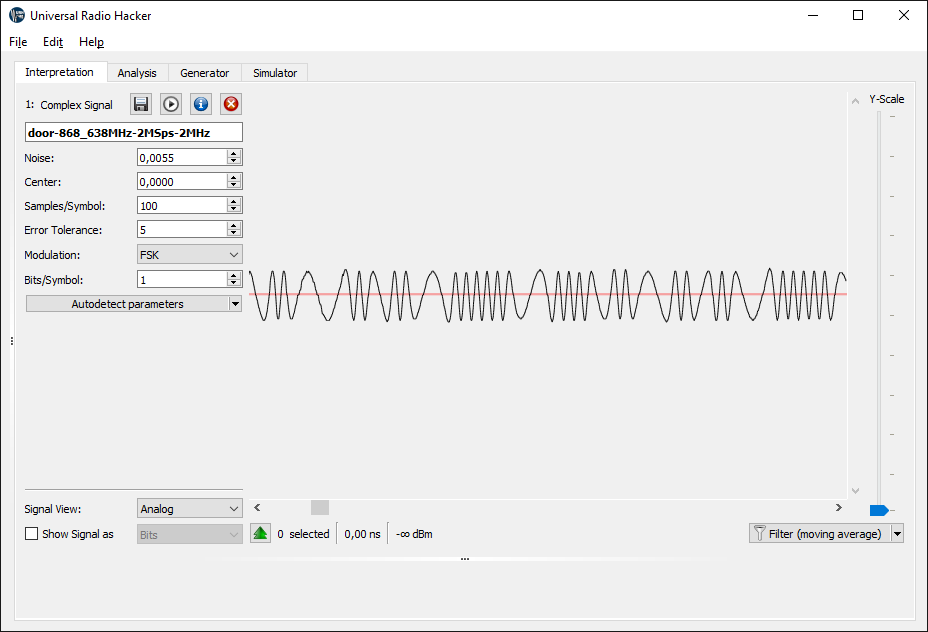
\includegraphics[width=0.9\textwidth]{images/6-pentesting/zoomed-in-signal.png}
    \caption{A cleanly captured RF signal, showing a clear sinusoidal pattern.}
    \label{fig:zoomed-in-signal}
\end{figure}

Lastly, once signals had been captured they could be replayed using URH's \textit{Send Signal} tool, see figure \ref{fig:uhr-replay-tool}. The tool lets you easily select and edit which parts of the captured signal to replay. Through a trial and error process, several combinations of packets were tested as a replay attack.
\begin{figure}[!ht]
    \centering
    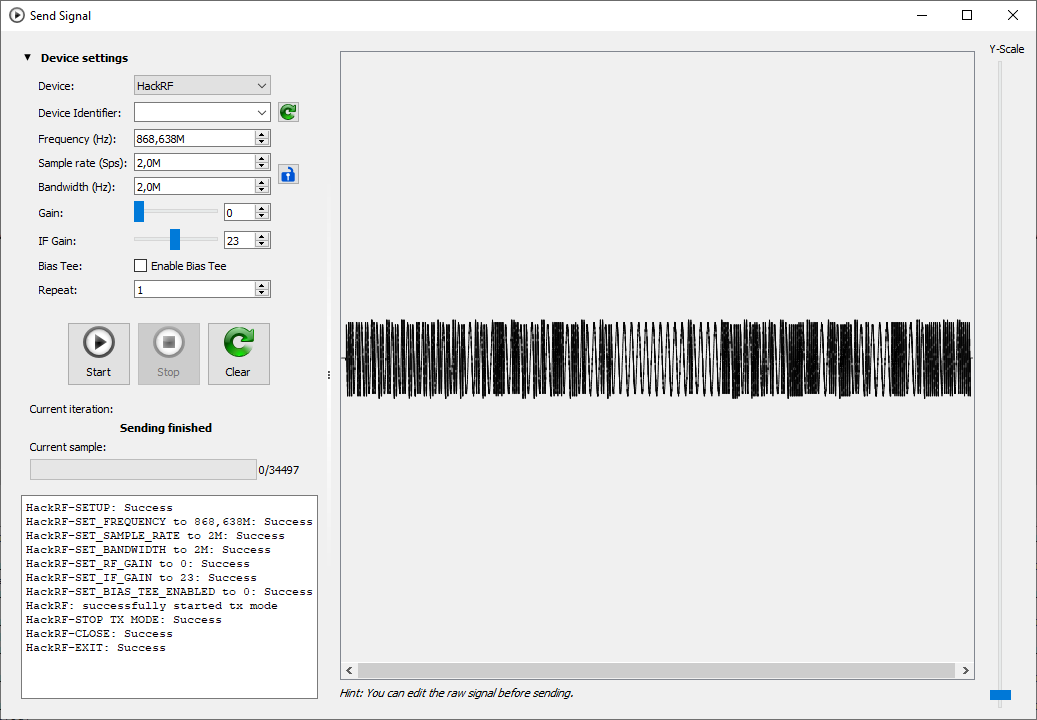
\includegraphics[width=0.9\textwidth]{images/6-pentesting/replay-signal.png}
    \caption{Performing a replay attack using Universal Radio Hacker.}
    \label{fig:uhr-replay-tool}
\end{figure}

\subsubsection{Results}
This test was successful and revealed \textit{critical} security flaws in the system. Every single tested endpoint of the RF communication were deemed vulnerable to replay attacks. The communication endpoints tested include the following:
\begin{itemize}
    \item Arming and disarming the alarm from the remote keypad.
    \item Triggering/resolving the tamper sensor of the door sensor.
    \item Triggering/resolving the tamper sensor of the camera.
    \item Triggering/resolving the tamper sensor of the main panel.
\end{itemize}
This has critical consequences for the security of the system. Capturing the RF signal of the user arming and disarming the alarm gives an attacker complete control of the arming state of the system. By simply replaying the signal, the main panel perceives this as a valid signal coming from the remote keypad.

\subsubsection{Discussion}
The system has no protection against replay attacks what so ever. This conclusion is strengthened by the fact that replaying the same signals several \textit{weeks} later was still successful. However, replaying the signals against a different system of the same model was tested and it was unsuccessful. Presumably, some kind of ID of the device is sent making the packets invalid for another copy of the system. It clearly shows, however, that the manufacturer Climax Technology either lacks the knowledge and competence to implement secure RF communication or have decided not to prioritize security at the RF layer. Either way this is a big mistake on their part which compromises the security of the whole system. SDRs have become much more available and much cheaper in the last few years. Attackers now have access to RF attacks which would have just a couple of years ago required very expensive and difficult to acquire hardware.

Furthermore, there are some factors that could potentially make this attack easier for an attacker in practice. When trying this attack signals were first incorrectly recorded at \texttt{868.0 MHz} instead of the correct frequency at \texttt{868.64 MHz}, giving rise to a very spiky signal. Still the replay attack worked using this signal without issue. This indicates that perhaps the signal does not have to captured that cleanly and that a badly captured signal, say from a distance or outside of the house, could be used to perform a replay attack. Presumably, the system implements some kind of error correction and noise filtering to increase the range and reliability of the RF communication. Additionally, regarding the tamper sensor signals, six signals are sent after one and other, see figure \ref{fig:rf-signal-capture}. However, replaying only one of them still yields a successful replay attack. All of the six packets work individually. Presumably, the system repeats the same or similar signal several times for redundancy, in case one gets lost or corrupted in transit. This means, however, that an attacker only has to capture one of them to be able to perform a replay attack. The reliability of capturing and transmitting the signals from a distance is, however, a bit unclear. This was not tested. On the other hand, an attacker could easily purchase an RF amplifier to increase their range and sensitivity.

The consequences of this vulnerability are huge. An attack can completely bypass the alarm, defeating the whole purpose of the system in the first place. By replaying a captured disarm signal the attacker can disarm the system, granting them access to the property without triggering an alarm. Additionally, replaying any of the other signals, namely triggering the tamper sensor, an attacker could trigger an alarm of an armed system without actually entering the premises. The owner would then get a message of an active breach and security personnel would be sent to the site. One could imagine an attacker repeatedly doing this until the owner perhaps thinks the system is broken and uninstalls it, at least temporarily, from the premises. At which point the premises would no longer be protected and an attacker could strike.
